\documentclass[10pt]{article}
\usepackage[margin=0.8in]{geometry}
\usepackage[T1]{fontenc}
\usepackage{lmodern}
\usepackage{microtype}
\usepackage{amsmath}
\usepackage{amsthm}
\usepackage{booktabs}
\usepackage{graphicx}
\usepackage{float}
\usepackage{hyperref}
\usepackage{xcolor}
\graphicspath{{./}}
\hypersetup{colorlinks=true,linkcolor=blue,citecolor=blue,urlcolor=blue}

\newtheorem{definition}{Definition}
\newtheorem{lemma}{Lemma}
\newtheorem{theorem}{Theorem}

\title{Deadlock-Free Minimal Adaptive Routing for a 3D Torus in Garnet}
\author{Lab 4 Project Report}
\date{\today}

\begin{document}
\maketitle

\begin{abstract}
This project adds parameterized 3D Mesh and 3D Torus topologies to gem5
Garnet and implements three routing modes: Mesh3D XYZ, Torus3D minimal
dimension-order routing (DOR), and a minimal adaptive Torus mode with a
one-way Mesh escape virtual-channel (VC) class. The default design reserves
one of four VCs as an escape path and keeps the other three adaptive. On the
4x4x4 transpose workload, it sustains 0.498859 packets/node/Ruby-cycle, versus
0.237455 for Torus DOR and 0.209570 for Mesh3D XYZ. A fixed-budget VC ablation
shows that one escape VC retains the performance of the unsafe no-escape upper
bound, while allocating more VCs to escape unnecessarily reduces throughput.
The report separates topology benefit from routing benefit and gives the
channel-dependency argument for progress.
\end{abstract}

\section{Goal and Scope}
The goal is not to present the 3D Torus as a new topology. Instead, this work
implements and evaluates congestion-aware minimal adaptive routing in Garnet,
where unrestricted adaptivity over Torus wrap channels can introduce cyclic
dependencies. The implementation uses a disjoint, connected 3D Mesh escape
subnetwork. Once a packet selects that class, it follows non-wrap XYZ routing
and never returns to an adaptive VC.

The evaluation uses 64 routers arranged as 4x4x4. Each Garnet physical
neighbour pair is represented by two directed internal links. The 3D Mesh has
$3(n-1)n^2=144$ undirected neighbour pairs at $n=4$; the 3D Torus has
$3n^3=192$, a 33.3\% increase. Therefore Mesh-versus-Torus results include
wrap-link cost and topology effects. Torus DOR versus Torus adaptive holds the
topology, link count, clocks, packet type, and total VC count fixed, so it
isolates the routing-policy effect.

\section{Implementation}
Router IDs use $zXY+yX+x$. The project adds \texttt{Torus3D.py} and
\texttt{Mesh3D.py}, command-line dimensions \texttt{--torus-x/y/z}, and these
routing-algorithm IDs:

\begin{center}
\begin{tabular}{cll}
\toprule
ID & Topology & Routing policy \\
\midrule
3 & Torus3D & Deterministic minimal XYZ DOR \\
4 & Torus3D & Minimal adaptive routing with Mesh escape VCs \\
5 & Mesh3D & Deterministic non-wrap XYZ \\
\bottomrule
\end{tabular}
\end{center}

Let $V$ be the number of VCs per vnet and $E$ the number of escape VCs. The
adaptive range is $[0,V-E)$ and the escape range is $[V-E,V)$. The
implementation validates $0 \le E < V$ for adaptive routing; safety requires
$E \ge 1$. New packets enter the adaptive range. At each adaptive hop, all
minimal Torus directions are considered, then candidates with the most usable
downstream adaptive VCs are preferred, with a pseudo-random tie break. If no
minimal adaptive output VC is usable, a head flit may enter an escape VC.

The escape route intentionally ignores Torus wrap links and advances signed
coordinates in X, then Y, then Z. This makes its path a route in a connected
3D Mesh. The switch allocator enforces the crucial one-way transition:
\[
  A\!\rightarrow\!A,\quad A\!\rightarrow\!E,\quad E\!\rightarrow\!E,
  \qquad\text{but never}\qquad E\!\rightarrow\!A.
\]

\begin{figure}[H]
\centering
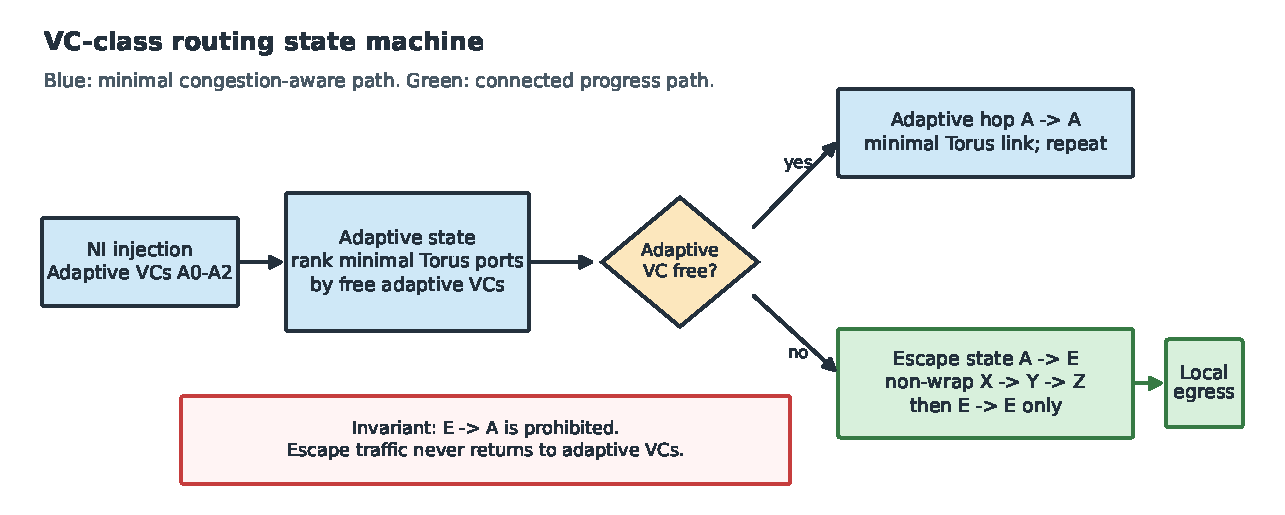
\includegraphics[width=0.94\linewidth]{routing_architecture.pdf}
\caption{Routing and VC-class state machine for the default 3A/1E split.
Blue is the performance path; green is the connected acyclic progress path.
The red transition is absent from the implementation.}
\label{fig:architecture}
\end{figure}

\section{Progress Argument}
The argument follows the connected acyclic escape-subset condition for adaptive
wormhole routing due to Duato~\cite{duato1995}. It is a proof about the route
and VC-allocation relation, not an inference from a finite simulation.

\begin{definition}[Escape channel set]
Let $C_E$ be all directed physical links paired with the Escape VC range. Its
channel-dependency graph (CDG) has one vertex per such channel and an edge
$c\rightarrow d$ if one legal Escape route can hold $c$ while requesting $d$.
\end{definition}

\begin{lemma}[Connectivity]
For every router pair $(s,t)$, a route using only $C_E$ exists.
\end{lemma}
\begin{proof}
The Escape policy changes the signed X coordinate until it equals the
destination X coordinate, then Y, then Z. Each step stays within the finite
non-wrap 3D Mesh, which is connected. The local egress terminates the route.
\end{proof}

\begin{lemma}[Acyclicity]
The CDG induced by $C_E$ is acyclic.
\end{lemma}
\begin{proof}
Within one dimension, an Escape route has a fixed sign and strictly advances
toward its destination; it cannot reverse or use a wrap link. It therefore
cannot make a same-dimension cycle. A dimension change is only X to Y or Y to
Z, never backwards. Order a dependency first by dimension (X, Y, Z), then by
coordinate progress in its fixed sign. Every legal CDG edge strictly advances
this lexicographic order, so a directed cycle is impossible.
\end{proof}

\begin{figure}[H]
\centering
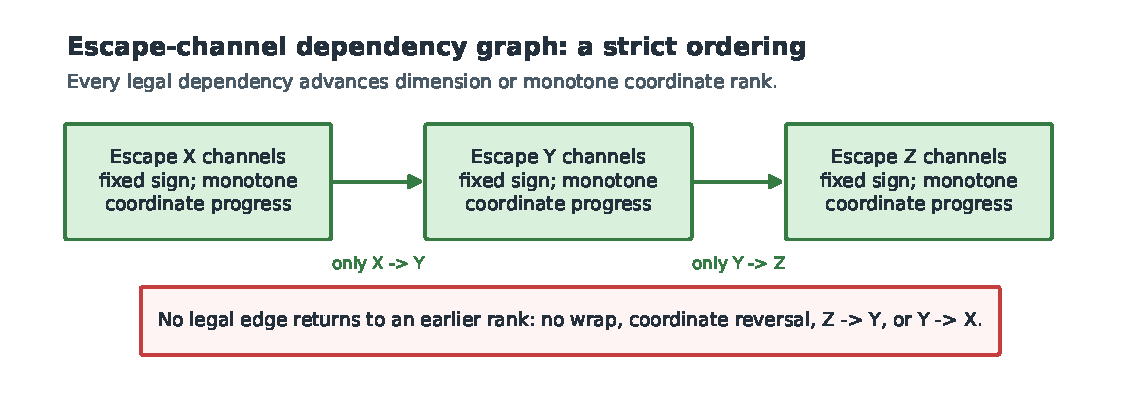
\includegraphics[width=0.88\linewidth]{escape_cdg.pdf}
\caption{Projection of the Escape-channel dependency graph. The omitted
backward and wrap dependencies are exactly what makes the subset acyclic.}
\label{fig:escape-cdg}
\end{figure}

\begin{theorem}[Deadlock freedom for $E\ge1$]
With a nonempty Escape range, the implemented route and VC-allocation relation
is deadlock-free, assuming finite buffers, reliable credits, and a fair switch
arbiter.
\end{theorem}
\begin{proof}
Assume a protocol deadlock exists. A blocked Escape header can request only its
next Escape channel: the allocator never assigns an Adaptive VC to an Escape
input. Following its wait dependencies can therefore never leave $C_E$; in a
finite deadlock it would contain a cycle in $C_E$, contradicting the preceding
lemma.

Now consider a blocked Adaptive header. If any minimal Adaptive output VC is
free, it can advance and is not deadlocked. Otherwise, the allocator tests its
unique non-wrap Escape next hop. If that Escape VC is free, it advances into
$C_E$. If it is occupied, its wait dependency enters $C_E$. Thus every
otherwise closed Adaptive wait set has an outgoing dependency into $C_E$.
Because the implementation contains no $C_E\rightarrow C_A$ assignment, a
finite dependency chain that enters $C_E$ cannot form an all-Adaptive cycle and
cannot form an Escape cycle by the acyclicity lemma. This contradicts the
assumed deadlock.
\end{proof}

The experiment with $E=0$ is deliberately labelled \emph{unsafe}. Completion
of a finite run without an escape class is not a proof of deadlock freedom.

\section{Methodology}
All main points use four VCs per vnet, single-flit vnet-0 control traffic, and
10,000 Ruby cycles. Ruby runs at 2 GHz and the system clock at 1 GHz. For
injection rate $r$ in packets/node/system-cycle, expected packets are
$N \cdot (\textit{simCycles}/2) \cdot r$. Throughput is received packets per
node per Ruby cycle; source acceptance is injected divided by expected packets.
A point is classified as stalled when source acceptance is below 0.9.

The 600-point sweep covers uniform random, 3D neighbour, 3D tornado, and 3D
transpose traffic. A separate X-opposite pattern sends $(x,y,z)$ to
$(x+X/2\bmod X,y,z)$ for even $X$, stressing equal-cost wrap-direction ties.
It is a useful validation traffic but does not replace the dependency argument.

\section{Results}
At low offered load, Torus routes reduce hop count relative to the Mesh. The
more important result occurs for transpose traffic, where adaptive routing
avoids deterministic route concentration. Table~\ref{tab:main} reports the
measured saturation summary.

\begin{table}[H]
\centering
\caption{Transpose traffic, 4x4x4, four VCs per vnet.}
\label{tab:main}
\begin{tabular}{lrrrr}
\toprule
Mode & Low-load latency & Hops & Max stable throughput & First stalled rate \\
\midrule
Mesh3D XYZ & 12.562 & 3.763 & 0.209570 & 0.48 \\
Torus3D DOR & 11.031 & 3.006 & 0.237455 & 0.50 \\
Torus3D adaptive/escape & 11.026 & 3.006 & 0.498859 & not observed \\
\bottomrule
\end{tabular}
\end{table}

The adaptive design reaches 2.38x Mesh throughput and 2.10x Torus DOR
throughput. The DOR comparison shows that the main high-load gain is not merely
the Torus wrap links: both Torus modes have the same links, yet only the
adaptive policy sustains the generator's maximum offered load.

\begin{figure}[H]
\centering

\includegraphics[width=0.91\linewidth]{latency_throughput.pdf}
\caption{Latency and delivered throughput for the four main traffic patterns.}
\end{figure}

\begin{figure}[H]
\centering
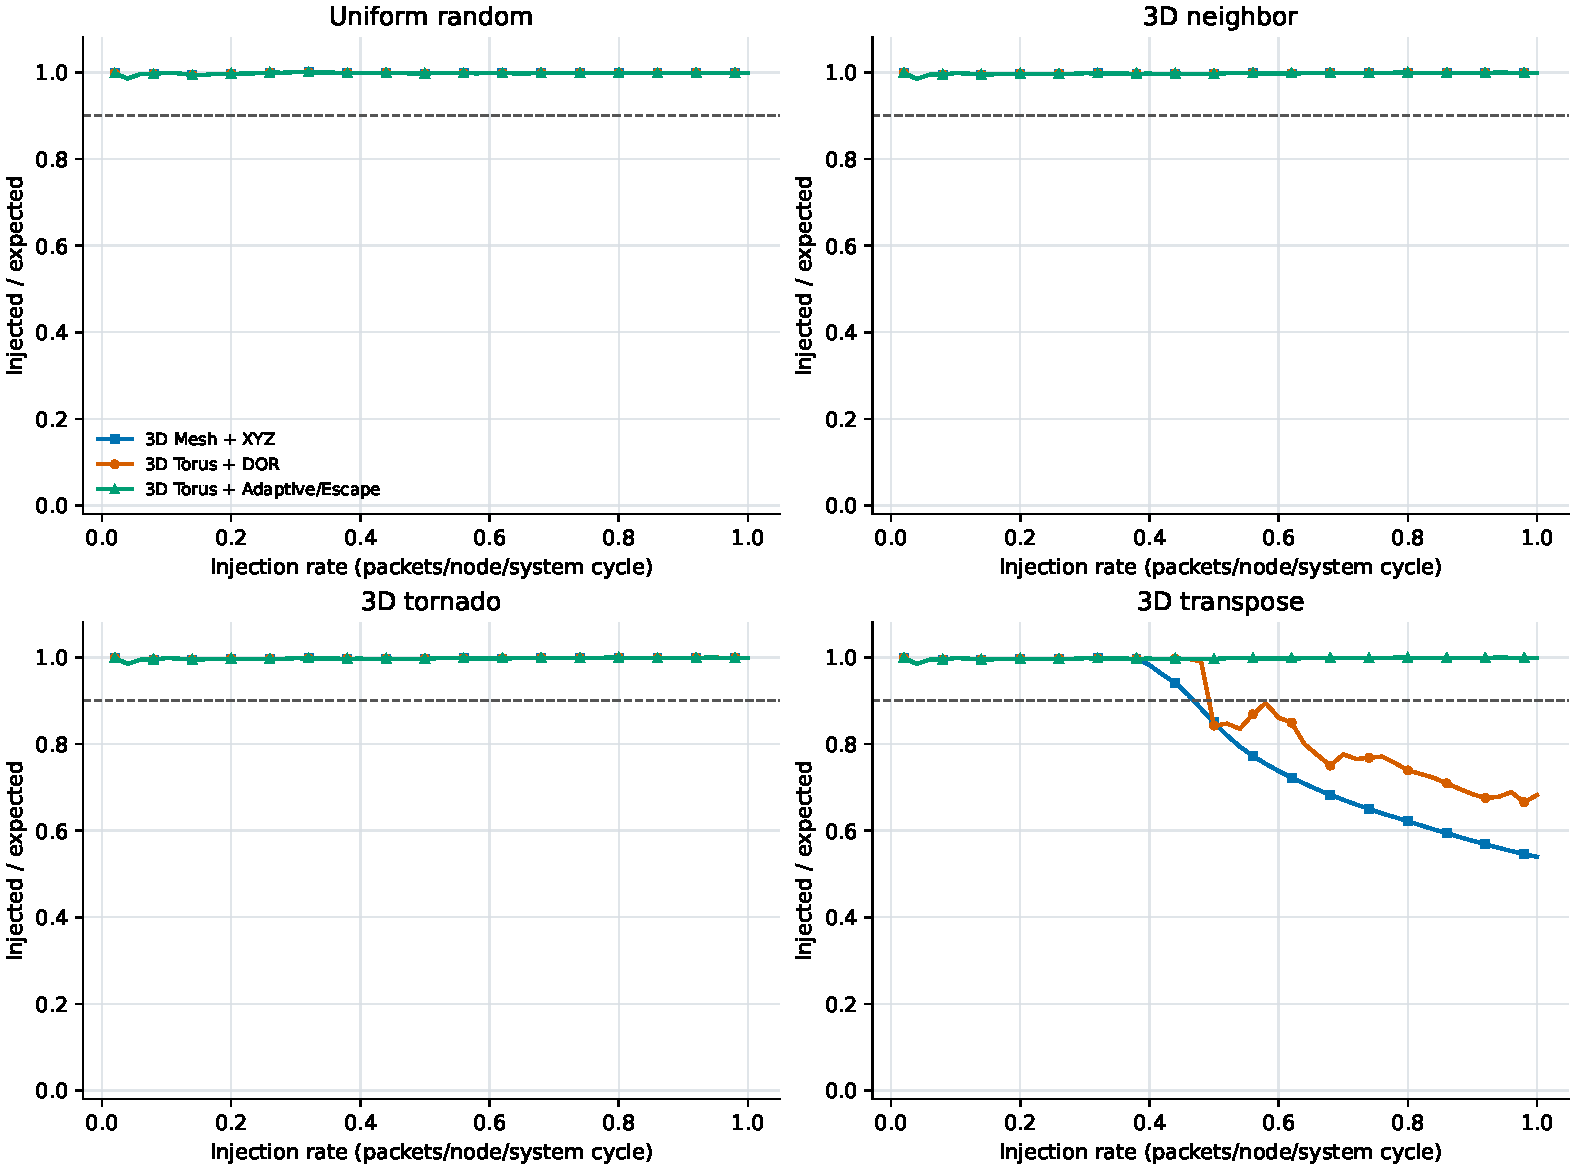
\includegraphics[width=0.91\linewidth]{source_acceptance.pdf}
\caption{Source acceptance distinguishes offered traffic from traffic that the NI can inject.}
\end{figure}

Escape use remains low at full offered load: 0.34\% of classified hops for
transpose, 0.52\% for uniform random, and 4.80\% for tornado. It is therefore
a rarely used progress path rather than the normal data path.

\section{Fixed-VC Ablation}
To test whether the default partition wastes resources, total VCs remain fixed
at four while the split varies. The no-escape result is a performance-only
upper bound; it intentionally carries no deadlock-freedom guarantee.

\begin{table}[H]
\centering
\caption{Transpose at injection rate 1.0, fixed total of four VCs.}
\begin{tabular}{crrrl}
\toprule
Adaptive/escape & Acceptance & Throughput & Latency & Safety guarantee \\
\midrule
4A/0E & 0.999 & 0.498866 & 11.782 & no \\
3A/1E & 0.999 & 0.498859 & 11.836 & yes \\
2A/2E & 0.773 & 0.386294 & 1138.807 & yes \\
1A/3E & 0.396 & 0.197884 & 3023.314 & yes \\
\bottomrule
\end{tabular}
\end{table}

\begin{figure}[H]
\centering
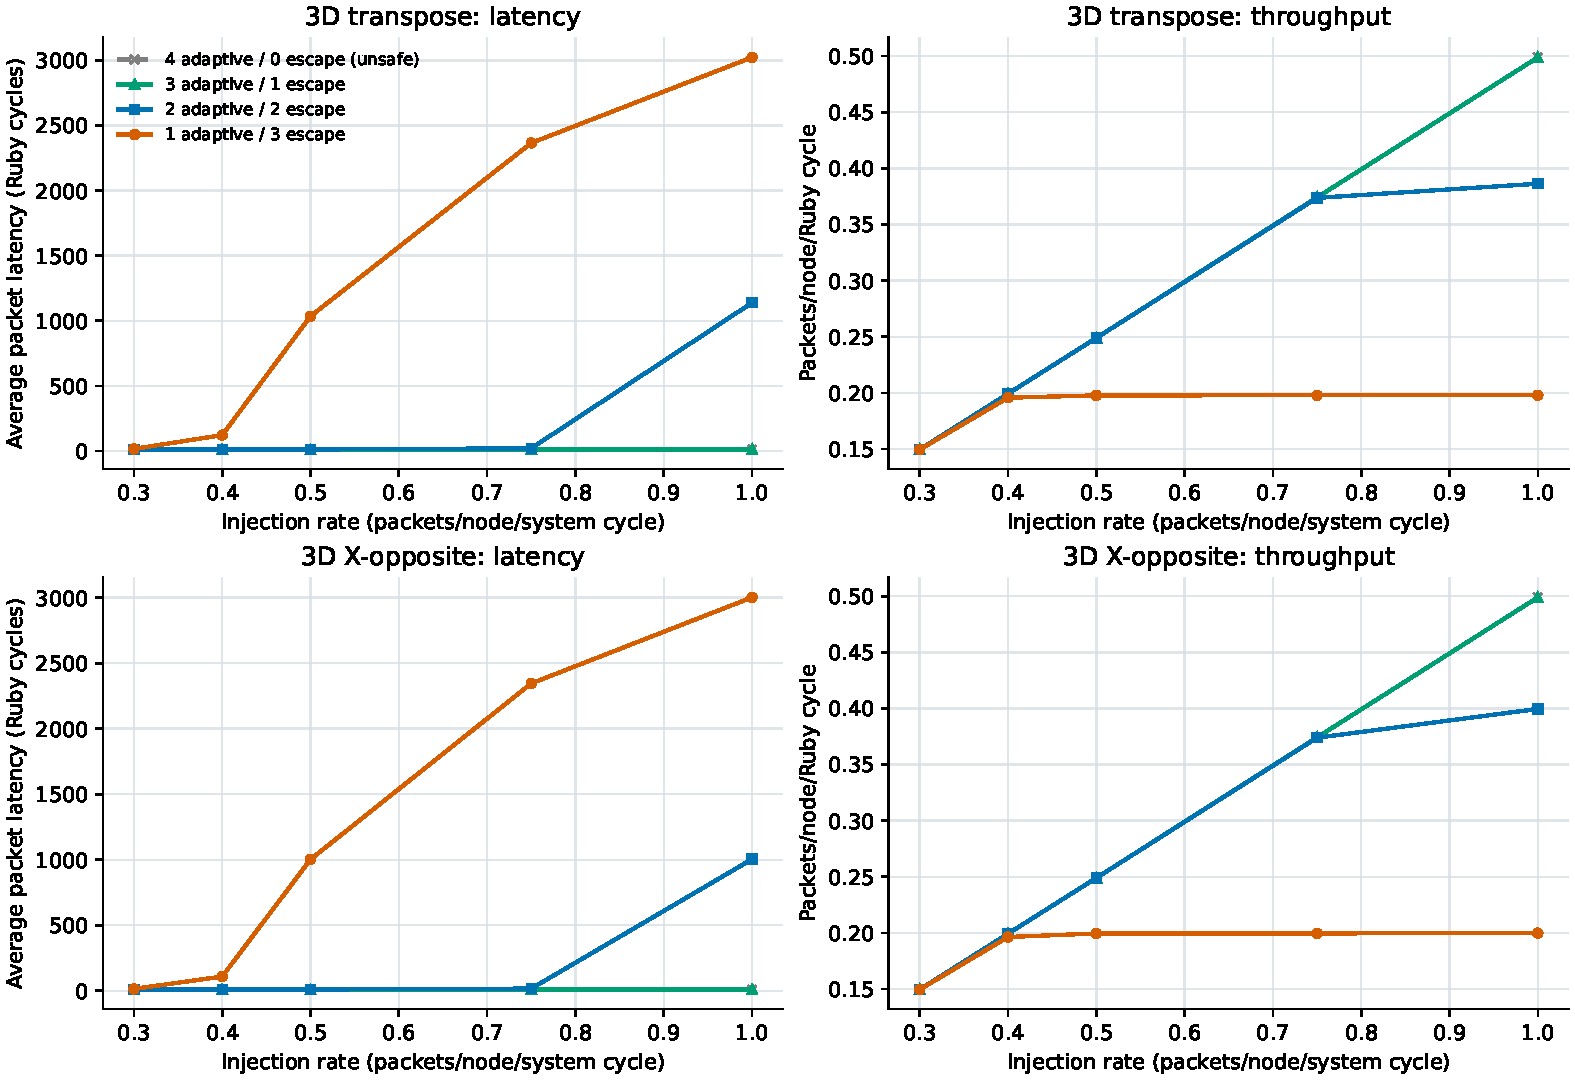
\includegraphics[width=0.94\linewidth]{vc_ablation.pdf}
\caption{Fixed-total-VC ablation under transpose and X-opposite traffic.}
\end{figure}

One escape VC is sufficient for the acyclic fallback and preserves the
no-escape throughput envelope. Reserving more escape VCs starves the adaptive
class, causing much earlier queueing and saturation. The X-opposite result
shows the same tradeoff, which makes 3A/1E the appropriate default.

\section{Additional Validation and Limitations}
The default split completed a 100,000-cycle X-opposite run at injection rate
1.0 with 0.998993 source acceptance, 0.999920 delivery ratio, 0.499456
throughput, and a 0.000989 escape-hop fraction. A vnet-2 five-flit tornado run
also completed in 10,000 cycles: 31,948 packets were injected and 31,885 were
received, with 478,737 adaptive hops, 110 escape hops, and 16 transitions.

The study uses synthetic traffic, one 4x4x4 size, deterministic simulator
seeding, and does not include area or power modelling. The link-count analysis
makes the Mesh/Torus resource difference explicit, but future work should add
multiple seeds, larger dimensions, application traces, and a router/link cost
model. The result is a functioning, reproducible Garnet implementation with a
routing-level progress argument, not a claim of a new 3D-Torus architecture.

\section{Reproduction}
From the repository root:
\begin{verbatim}
./.venv/bin/python lab/lab4/run_sweep.py
./.venv/bin/python lab/lab4/plot_results.py
./.venv/bin/python lab/lab4/run_vc_ablation.py --force --jobs 3
./.venv/bin/python lab/lab4/plot_vc_ablation.py
./.venv/bin/python lab/lab4/draw_diagrams.py
cd lab/lab4 && pdflatex report.tex
\end{verbatim}
The CSV files, figures, and scripts are kept in \texttt{lab/lab4/}; raw logs
are kept under the ignored \texttt{lab/lab4/artifacts/} directory.

\begin{thebibliography}{1}
\bibitem{duato1995}
J. Duato, ``A Necessary and Sufficient Condition for Deadlock-Free Adaptive
Routing in Wormhole Networks,'' \emph{IEEE Transactions on Parallel and
Distributed Systems}, vol. 6, no. 10, pp. 1055--1067, 1995.
\end{thebibliography}

\end{document}
